\chapter{Computing Fundamentals in LabVIEW}
In this chapter, we will go over some of the basic building blocks of a computer program in the context of $\labview$. This chapter will be heavy on examples in $\labview$, but will be light on the trivial details such as how to open a VI and how to place functions and controls. If you have not already done so, review the exercise in section \ref{HowToPlace} in Chapter 1.\\

If you get stuck, you may open the $\labview$ help files my pressing \texttt{Ctrl+?} and navigating to the ``Fundamentals'' section. If you would like to see more examples of how things are done in $\labview$, on the taskbar select ``Help'' and navigate down the menu to find ``Find Examples...'', here you will find a library of examples. These examples range from trivial arithmetic, to programs which would make you a cup of coffee if you supply it with enough hardware.

\section{Decision making structures}
Without the ability to make decisions, computers would not be as useful as they are now. Try to think of a computer program that makes no decisions based on it's input, they do exist and some are even useful. We are not interested in such academic programs, we want our computer to do the heavy lifting for us, just imagine clicking \texttt{yes} or \texttt{no} for a data set of a billion numbers. My computer can do that in $5.76$ seconds (I just checked using $\labview$).\\

If you are familiar with programming, you know that the most fundamental decision making block is an ``if-statement''. You supply the block with a condition, and the program executes statements based on that condition. Technically speaking, $\labview$ has no such thing as an if-statement, it has ``case-structures'' and ``ternary-operators''.

\subsection{Case Structures}
The case structure executes a block of code according to its input condition. In $\labview$, the input condition may be either a boolean value, an enumeration, or an error value. Figure \ref{ch2egTrue} (A) shows how a case structure looks, a thick grey box with a green \texttt{?} and a selection box stating ``True''. What ever is inside this grey box will be executed if a boolean true value is wired into the conditional terminal, the green \texttt{?}. Figure \ref{ch2egFalse} shows what would be executed if the condition is false.\\
\begin{figure}
	\centering
	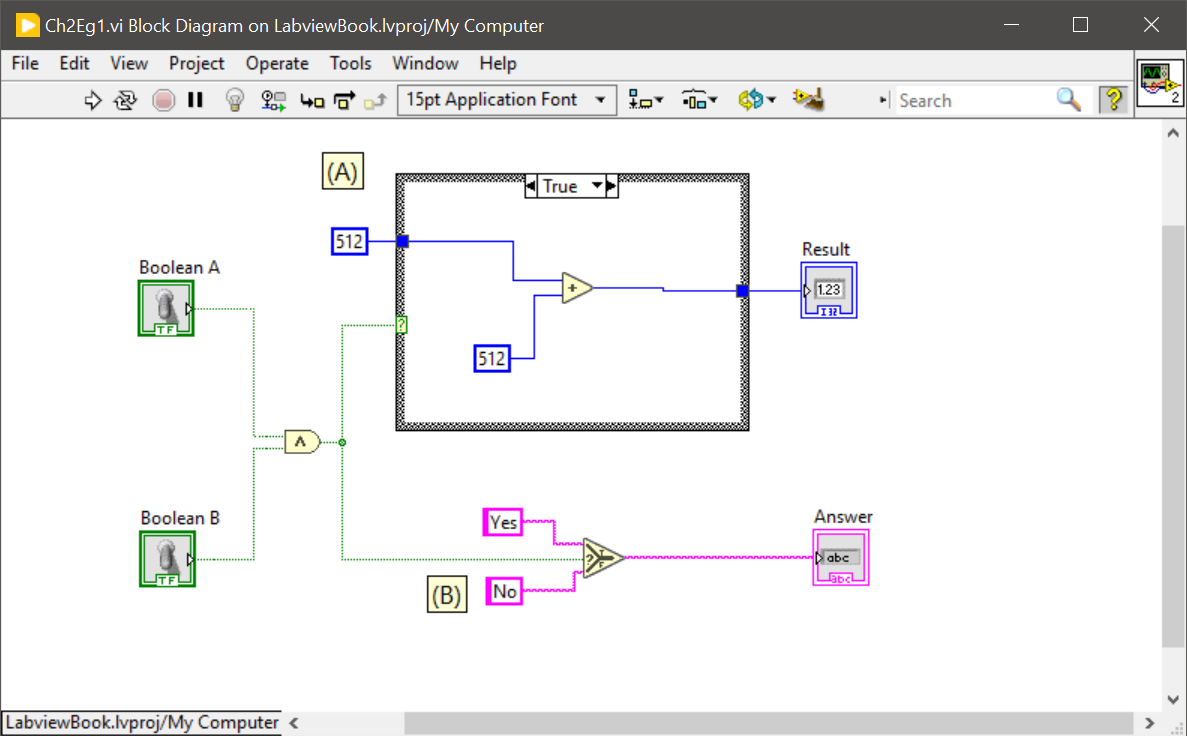
\includegraphics[width=\textwidth]{ch2eg1True}
	\caption{A case structure showing its truth block (A), and a ternary operator (B).}
	\label{ch2egTrue}
\end{figure}
\begin{figure}
	\centering
	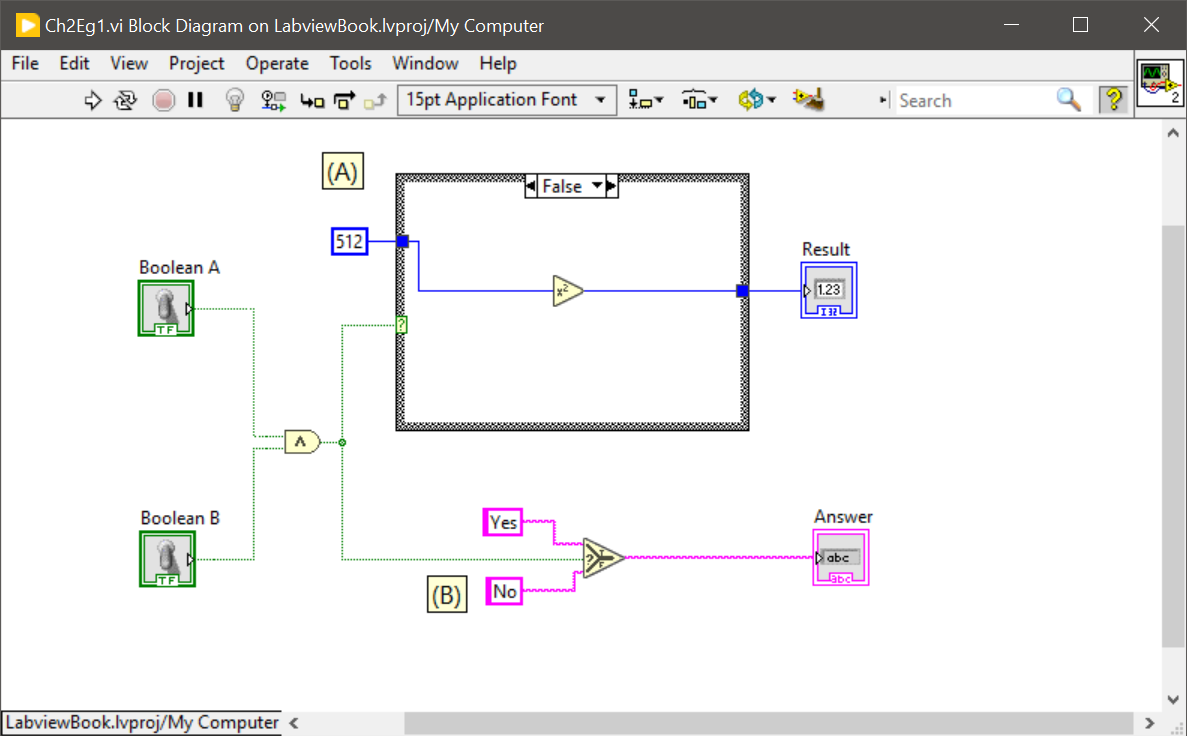
\includegraphics[width=\textwidth]{ch2eg1False}
\caption{A case structure showing its false block (A), and a ternary operator (B).}
\label{ch2egFalse}
\end{figure}

Comparison functions in $\labview$ produce only boolean values, this you have seen in the examples so far. Feeding these boolean values into case structures allow you to select different operations to be preformed. The example provided in figures \ref{ch2egTrue} \& \ref{ch2egFalse} show how you would choose two different operations on an integer. If the condition is true, 512 is added to the input number and the result is given, the indicator outside the case structure.  If the value is false, 512 is squared and the result given.\\

A case structure also accepts enumeration values. This is similar to a switch structure in \texttt{C} programming. In figure \ref{ch2eg2}, a value named ``Multiply'' is placed into the case structure. This allows you to have many paths of execution in a single structure. In the example, a simple calculator is made which takes two input numbers and an enumeration condition, the block then executes the proper logic and hands you the result at the end. One of the mini projects at the end of this section chapter will require you to create a 4-function calculator.\\
\begin{figure}
	\centering
	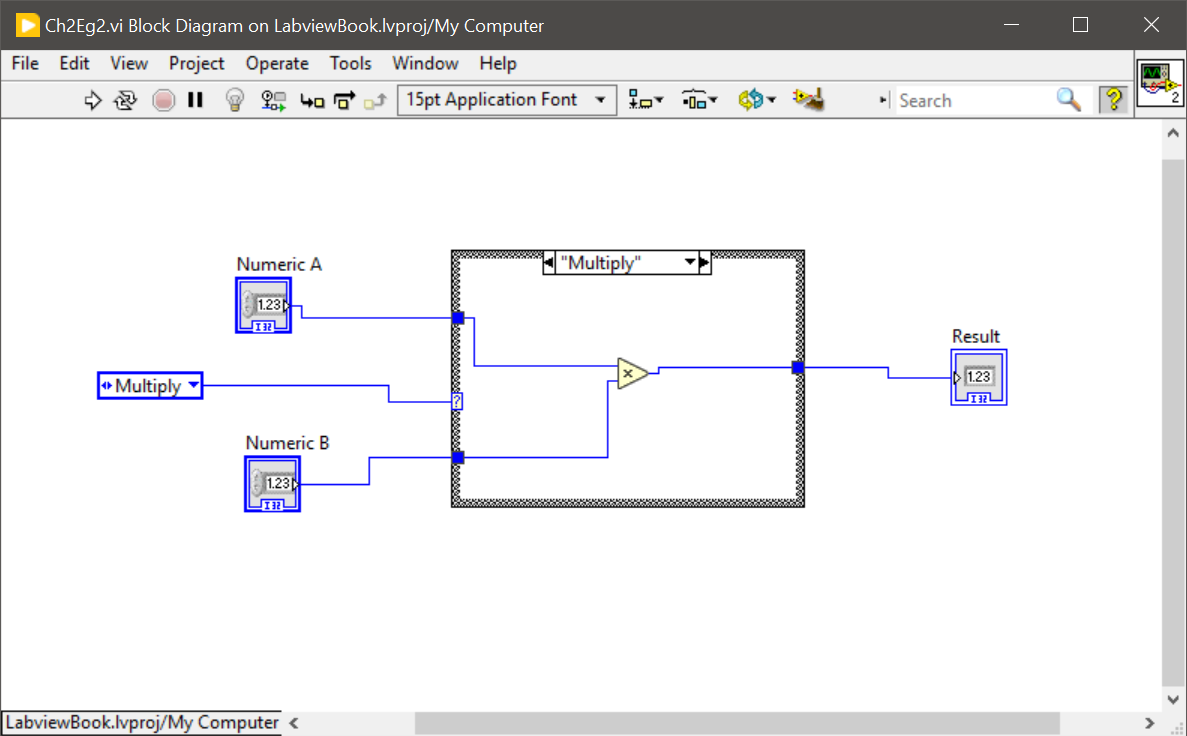
\includegraphics[width=\textwidth]{ch2eg2}
\caption{A simple calculator using an enumeration type and a case structure.}
\label{ch2eg2}
\end{figure}

\subsection{Ternary operators}
The plural in the title is misleading, there is only one ternary operator in $\labview$. Figure \ref{ch2egTrue} (B), on page \pageref{ch2egTrue}, is this little function in action. You supply it with a boolean value and outputs either its truth or false value. In this example, if the boolean value is true, then the ternary operator outputs the string ``Yes''.\\

The only caveat is that you must use the same variable type for its true and false inputs, this type will also be its output type.  There really isn't anything more special about the ternary operator. It is possible to implement a ternary operator using a case structure, an exercise left for the reader.

\section{Code looping structures}
In the previous section, I mentioned that my computer could make a billion decisions in $5.76$ seconds. The program certainly did not contain a billion case structures, it only had one.\\

It is quite rare for a program to only make one decision before execution stops, most probably you have a few decisions which would need to be repeated thousands of times per execution. One may even say that you would like to have a program perform a ``loop'' of decisions. This is were loop structures come into play.\\

The two loop structures available to us in $\labview$ is the ``For Loop'' and the ``While Loop''. The for loop executes a set number of times while the while loop executes until some specified condition is met. These two structures are closely related however since the for loop can pretend to be a while loop. It is also worth mentioning in passing, to those of you with previous programming experience, that both loops act as `do-while'' loops since they execute at least once before evaluating their conditional terminals.\\

The flow of information in $\labview$ is rather unconventional, this will be elaborated upon in a future section, but for now there will be references to arrays, time functions, and shift registers without going into depth for either topics.

\subsection{For Loops}
A for loop executes a predetermined amount of times. Figure \ref{ch2eg3} is perhaps the most simple, yet interesting, loop possible in $\labview$. You set the number of times the loop should run in the ``Number of times'' control and the loop shows you the iteration step number along with a random floating point number between 0 \& 1. The little watch function in the bottom right corner is to slow the loop execution speed to twice every second so you are able to observe the number generated.\\

The example is heavily constrained however, there is no way for the information generated to be stored in memory so there is no knowlage for what the random number was in the previous iteration let alone what the series of generated numbers were.\\

Just by introducing a concept known as a shift register, we can actually start making useful programs, or what ever useful means in this case. A shift register allows you to store a variable from a current loop iteration so that it is useable in the next iteration. To illustrate this, let us create a loop that prints out, in sequence, the first 10 numbers in the Fibonacci sequence.\\

The Fibonacci sequence, defined by the recurrence relation:
\begin{equation*}
	F_0=0,\quad F_1=1,\quad F_n= F_{n-1} + F_{n-2}
\end{equation*}
An implementation of this may be found in figure \ref{ch2eg4}. On the right hand side of the loop structure is a little blue arrow in a box, this is the terminal where you value the number you want available to the next loop iteration. To add a shift register to a loop, \texttt{right click} on any side of the loop frame and select ``Add Shift Register'' from the drop-down menu.\\

You may notice in that example that the left hand side has two little arrows stacked on top of each other, this gives you access to the previous iteration values. In this case the top arrow is the value of iteration n-2 and the bottom arrow is the value of iteration n-1. You can extend or reduce the number of iterations available by clicking and dragging the bottom edges of the shift register.\\
\section{Aggregate data types}

\section{Creating functions}

\section{Slightly more advanced Mini Projects}